\documentclass[border=2pt,tikz]{standalone}



\usetikzlibrary{decorations.pathmorphing}
\begin{document}
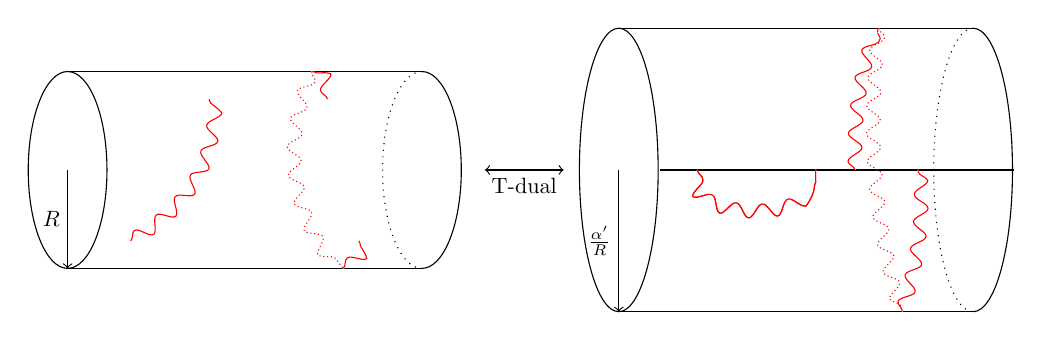
\begin{tikzpicture}[remember picture]
\draw (0,0) ellipse (0.5 and 1.25);
\draw (0,-1.25) -- (4.5,-1.25);
\draw (4.5,-1.25) arc (-90:90:0.5 and 1.25);
\draw [dotted] (4.5,1.25) arc (90:-90:-0.5 and 1.25);
\draw (0,1.25) -- (4.5,1.25);
\draw[->] (0,0)  to  node [left,scale=0.8] {$R$}  (0,-1.25);
\draw[<->] (5.3,0)  to  node [below,scale=0.8] {T-dual}  (6.3,0);

\tikzset{
    demo decoration/.style={
        white,
        postaction={draw=red,decorate,decoration=#1}
    }
}  
    \draw[demo decoration=snake](.8,-.9)to[bend right](1.8,.9);
    \draw[demo decoration=snake](3.3,.9)to[bend right](3.1,1.25);
     \draw[demo decoration=snake,densely dotted](3.1,1.25)to[bend right](3.5,-1.25);
    \draw[demo decoration=snake](3.5,-1.25)to[bend right](3.7,-.9);
    
\draw (7,0) ellipse (0.5 and 1.8);
\draw (7,-1.8) -- (11.5,-1.8);
\draw (11.5,-1.8) arc (-90:90:0.5 and 1.8);
\draw [dotted] (11.5,1.8) arc (90:-90:-0.5 and 1.8);
\draw (7,1.8) -- (11.5,1.8);
\draw[->] (7,0)  to  node [left,scale=0.8] {$\frac{\alpha'}R$}  (7,-1.8);

\draw (7.52,0) -- (12.02,0);


    \draw[demo decoration=snake](8,0)to[bend right=100](9.5,0);
    \draw[demo decoration=snake](8,0)to[bend right=100](9.5,0);

    \draw[demo decoration=snake](10,0)to[bend left=10](10.3,1.8);
     \draw[demo decoration=snake,densely dotted](10.3,1.8)to[bend right=10](10.6,-1.8);
    \draw[demo decoration=snake](10.6,-1.8)to[bend right=10](10.8,0);


\end{tikzpicture}
\end{document}